%!TEX root = pfc-memoria.tex
%!TEX encoding = UTF-8 Unicode

\chapter{Diseño de la solución}

\epigraph{``La función de un buen software es hacer que lo complejo aparente ser simple.''}{\textsc{Grady Booch} (1955--)}

En este capítulo comentamos las decisiones de diseño tomadas para la construcción de la aplicación teniendo en cuenta la ERS del \fullref{chap:analisis-requisitos}.

\section{Patrón de diseño}

Como la aplicación será una aplicación de escritorio, con su interfaz gráfica de usuario (GUI), diseñaremos el sistema de manera adecuada para dar soporte a un desarrollo rápido de la aplicación dirigida por eventos \emph{(Event-driven programming).}\index{EDP}\index{Event-driven programming@\emph{Event-driven programming}}

Se diseñará un sistema basado en el patrón Modelo-Vista-Presentador (MVP, \emph{Model-View-Presenter} en inglés)\index{MVP}\index{Modelo-Vista-Presentador}\index{Model-View-Presenter@\emph{Model-View-Presenter}}. Es un patrón parecido al conocido Modelo-Vista-Controlador (MVC, \emph{Model-View-Controller} en inglés)\index{MVC}\index{Modelo-Vista-Controlador}\index{Model-View-Controller@\emph{Model-View-Controller}}, sin embargo presenta algunas diferencias que cabe destacar (véase \autoref{fig:MVP-MVC}):

\begin{itemize}
\item En el MVP, el Controlador pasa a llamarse Presentador, y se define como un Controlador-supervisor, colocándose como hombre-en-el-medio (mitm, \emph{man-in-the-middle})\index{mitm}\index{man-in-the-middle@\emph{man-in-the-middle}} entre la Vista y el Modelo.
\item Así, el Modelo no puede interactuar con la Vista de manera directa, sino sólo a través del Presentador.
\item Esto permite mayor independencia de código y mayores oportunidades de reutilización, al ser más sencillo cambiar la Vista por otra sin afectar al Modelo, que contiene el acceso a la información y la lógica de negocio.
\end{itemize}

\begin{figure}[htbp]\centering
\begin{subfigure}[b]{0.49\textwidth}\centering
\includegraphics[width=0.85\textwidth]{MVC}
\caption{Modelo-Vista-Controlador (MVC)}
\end{subfigure}
\begin{subfigure}[b]{0.49\textwidth}\centering
\includegraphics[width=0.94\textwidth]{MVP}
\caption{Modelo-Vista-Presentador (MVP)}
\end{subfigure}
\caption[Patrones MVC y MVP]{Patrones MVC y MVP. La principal diferencia en MVP es que el Modelo no puede interactuar con la Vista si no es a través del Presentador. \\
{\footnotesize \url{http://www.gwtproject.org/articles/testing_methodologies_using_gwt.html}}}
\label{fig:MVP-MVC}
\end{figure}

\section{Arquitectura del sistema}

La aplicación se desarrolla usando el lenguaje de programación Python~3.

En la \fullref{fig:architecture} se encuentra un resumen visual de la situación de cada componente dentro del patrón MVP y la colaboración entre ellos.
Los componentes (todos de software libre) que se reutilizan son:
\begin{description}
\item[Qt5]\index{Qt} Biblioteca de herramientas gráficas para la creación de interfaces de usuario ---con licencia de software libre--- en C++ que proporciona widgets y un framework de desarrollo de GUI compatible con la programación dirigida por eventos, soportado por las plataformas Windows, GNU/Linux y Mac~OS~X, entre otros \citep{Huang2015}. Actualmente mantenido por Digia.
\item[PyQt5] Puente \emph{(binding)} entre Python~2/3 y la biblioteca Qt5, mantenido por Riverbank Computing \citep{Summerfield2008}.
\item[QML] \emph{Qt Markup Language}\index{QML} es un motor declarativo de interfaces de usuario para Qt con sintaxis compatible con ECMAScript, integrado dentro de las versiones modernas de Qt5 \citep{web:QmlBook}.
\item[NLTK3] \emph{Natural Language Toolkit}\index{NLKT} es una biblioteca de utilidades en procesamiento de texto para Python \citep{Perkins2014}.
\item[scikit-learn] Biblioteca en Python para aprendizaje automático \citep{Pedregosa2011}.
\item[NumPy] Biblioteca en Python/C++ para el tratamiento de vectores/matrices numéricos y precisión arbitraria de manera eficiente desde Python \citep{Bressert2012}.
\end{description}

Los componentes a desarrollar son dos módulos en Python, uno para cubrir el \fullrefSRSObj{biblioteca-nlp-ml}, y el segundo módulo para el \fullrefSRSObj{gui}; y que se describen a continuación:
\begin{description}
\item[\codep{pfcsamr.gui}] Implementa el Presentador que recibe y maneja los eventos generados por el usuario al interactuar en el GUI, y canaliza las operaciones comandadas hacia el Modelo. Así mismo, monitoriza los cambios que se produzcan en el Modelo y refleja estos cambios en el GUI actualizando el estado de la pantalla. Este modelo incluye también la descripción de la interfaz en el lenguaje declarativo QML.\index{QML}
\item[\codep{pfcsamr.orchestrator}] Implementa el Modelo que actúa «orquestando» todo el proceso de análisis de sentimiento, coordinando de manera coherente los paquetes de NLTK3 y scikit-learn, y ofreciendo toda la funcionalidad de E/S.
\end{description}

Los componentes a desarrollar se indican en color verde en la \autoref{fig:architecture}, mientras el resto son componentes proporcionados por proyectos de software libre disponibles públicamente.

\begin{figure}[htbp]
\centering
\vspace{0.5cm}
\resizebox{0.75\textwidth}{!}{\input{architecture.puml.tex}}
\caption{Diagrama de arquitectura de componentes}
\label{fig:architecture}
\end{figure}


\section{Clases}

\section{Secuencias}




\resizebox{0.5\textwidth}{!}{\input{diag1.puml.tex}}

\ldots

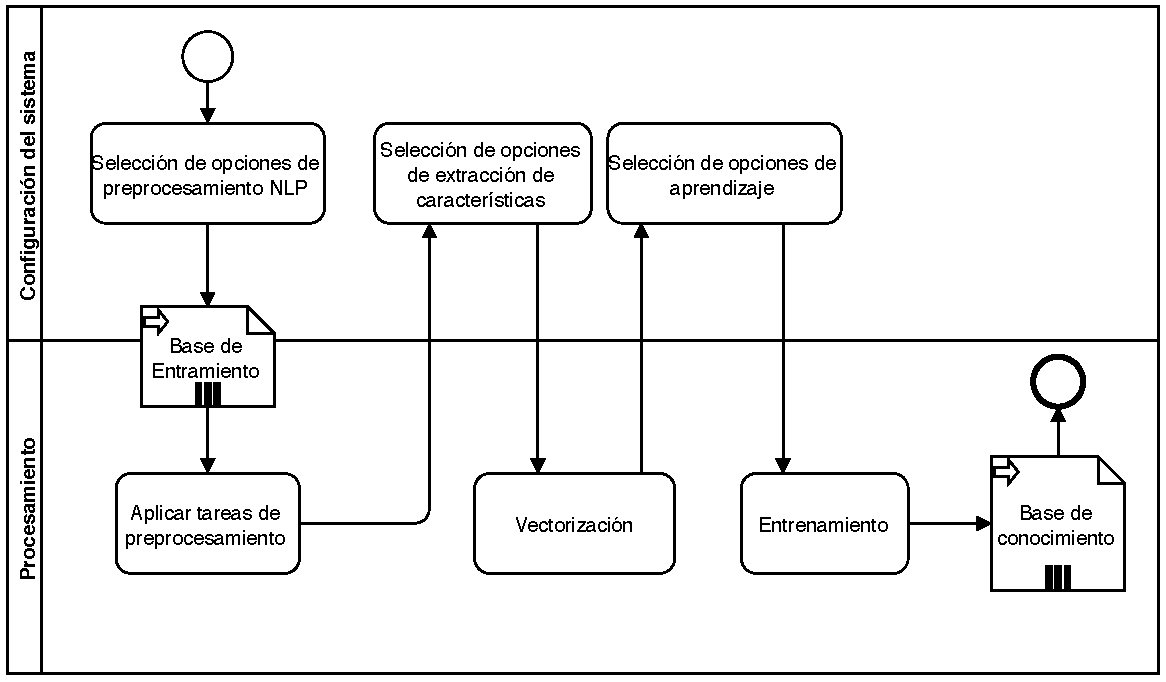
\includegraphics[width=\textwidth]{bpmn-entrenamiento}

\ldots

\includegraphics[width=14cm]{gui-1-load}

\ldots

\includegraphics[width=12cm]{gui-2-preprocess}

\ldots

\includegraphics[width=12cm]{gui-3-features}

\ldots

\includegraphics[width=12cm]{gui-4-learn}

\ldots

\includegraphics[width=12cm]{gui-5-classify}

\ldots
